%%%%%%%%%%%%%%%%%%%%% chapter.tex %%%%%%%%%%%%%%%%%%%%%%%%%%%%%%%%%
%
% sample chapter
%
% Use this file as a template for your own input.
%
%%%%%%%%%%%%%%%%%%%%%%%% Springer-Verlag %%%%%%%%%%%%%%%%%%%%%%%%%%


\chapter{Needle Localization in MR Images}
\label{sec:mritracking} % Always give a unique label
% use \chaptermark{}
% to alter or adjust the chapter heading in the running head

The purpose of this experiment is to validate the parametric curve fit and needle model on imagery representative of what would be available from intraoperative imagery during an MRI-guided insertion.

Assumptions about needles and conditions of insertion:
\begin{itemize}
\item A single beveled-tip clinical-style biopsy needle is inserted and tracked.
\item The initial vector of the needle is normal to the axial plane.
\item Only homogeneous gelatin or plastic tissue phantoms are used during experiments. The problem of identifying the needle in the presence of anatomy or other clutter is not addressed.
\end{itemize}

\section{Software Architecture}
\subsection{Simulated MRI Scanner}
Full 3D MRI volumes take a long time to produce, especially if high resolution is desired: the scan time for each volume used in this experiment was approximately 5 minutes. This is a prohibitively long time in the context of real-time intraoperative imaging, so the MRI would be configured to provide 2D scans in requested planes with limited field of view. To simulate this functionality, a  Slicer module was created to resection 2D slices from each 3D volumes at specified depths.

\subsection{Needle Tracking Module}
A second Slicer module manages the needle tracking process. Figure \ref{fig:MRI_architecture} shows the architecture of this module relative to the Slicer environment and the needle modeling utility. A linear transform node is set to match the pose of the needle base in each saved volume. When commanded by the operator, the module requests slices of the MRI volume at evenly-spaced coordinates along the shaft of the needle. The needle position in each section is calculated as the centroid of the thresholded region closest to the estimated position of the needle provided by the previous needle model curve. The position of the needle base is appended to this list of needle coordinates, and the combined list is used as one of the inputs for the needle curve optimization.

\begin{figure}[h]
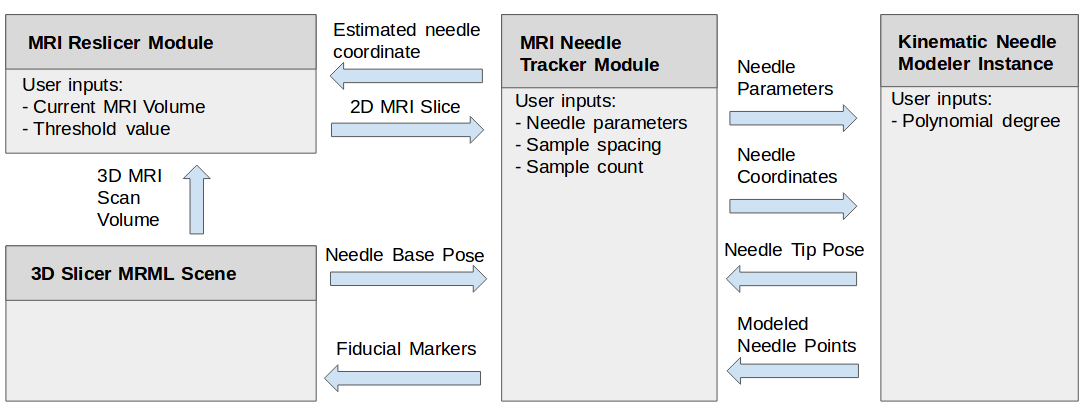
\includegraphics[width=1.0\textwidth]{Fig/chap5/MRI_software_architecture.png}
\caption{System architecture for needle detection and modeling from MRI data.}
\label{fig:MRI_architecture}
\end{figure}

% \begin{algorithm}
% \caption{Needle Tracking in MRI}\label{alg:mri_tracking}
% \begin{algorithmic}[1]
% \Procedure{Track Needle}{$coords_{needle},L_{needle},poly_{prev}$}
% \State $t \gets CalculateParameters(coords_{needle}, L_{needle})$
% \If {$poly_{prev} is None$}
% 	\State $poly_{init} \gets LeastSquares(coords_{needle})$
% \Else
% 	\State $poly_{init} \gets poly_{prev}$
% \EndIf
% \State $cons \leftarrow DefineConstraints(t, coords_{needle}, L_{needle})$
% \State $poly_{opt} \gets DoOptimization(poly_{init}, cons)$
% \State \textbf{return} $poly_{opt}$
% \EndProcedure
% \end{algorithmic}
% \end{algorithm}

\section{Experiment}
\subsection{MRI Data Collection}
Two series of MRI volumes were captured in the 3T scanner at UMass Medical Center using a 3D Fast Field Echo protocol. The dimensions of each voxel are 0.4mm x 0.4mm x 0.5mm. The phantoms used were made of agar gelatin. The needle was a 150mm stainless steel (E = 200 GPa) clinical-style biopsy needle with a beveled tip and a diameter of 2mm. Removable plastic spacers with a thickness of 5.95mm regulated the insertion distance. In Insertion A two spacers were removed between scans, so the needle moves in increments of 11.9mm. In Insertion B one spacer was removed between scans, so the needle moves in increments of 5.95mm. The plastic alignment frame shown in Figure \ref{fig:needle_guide} kept the needle aligned along a known vector relative to the phantom. When used in conjunction the alignment frame and spacers allow the 6-DOF pose of the needle base to be calculated in each scan without the use of a Z-frame or external tracking equipment.

\subsection{Needle Localization}
Each volume was thresholded at intensity 1500 to isolate the needle artifact. The segmentation labelmap was exported and processed separately.

The MRI volumes for each insertion step were loaded in sequence and a linear transform was set to match the pose of the needle base at each step. The needle localization algorithm was run on each dataset in turn to generate an array of points representing the simulated needle.

\begin{figure}[h]
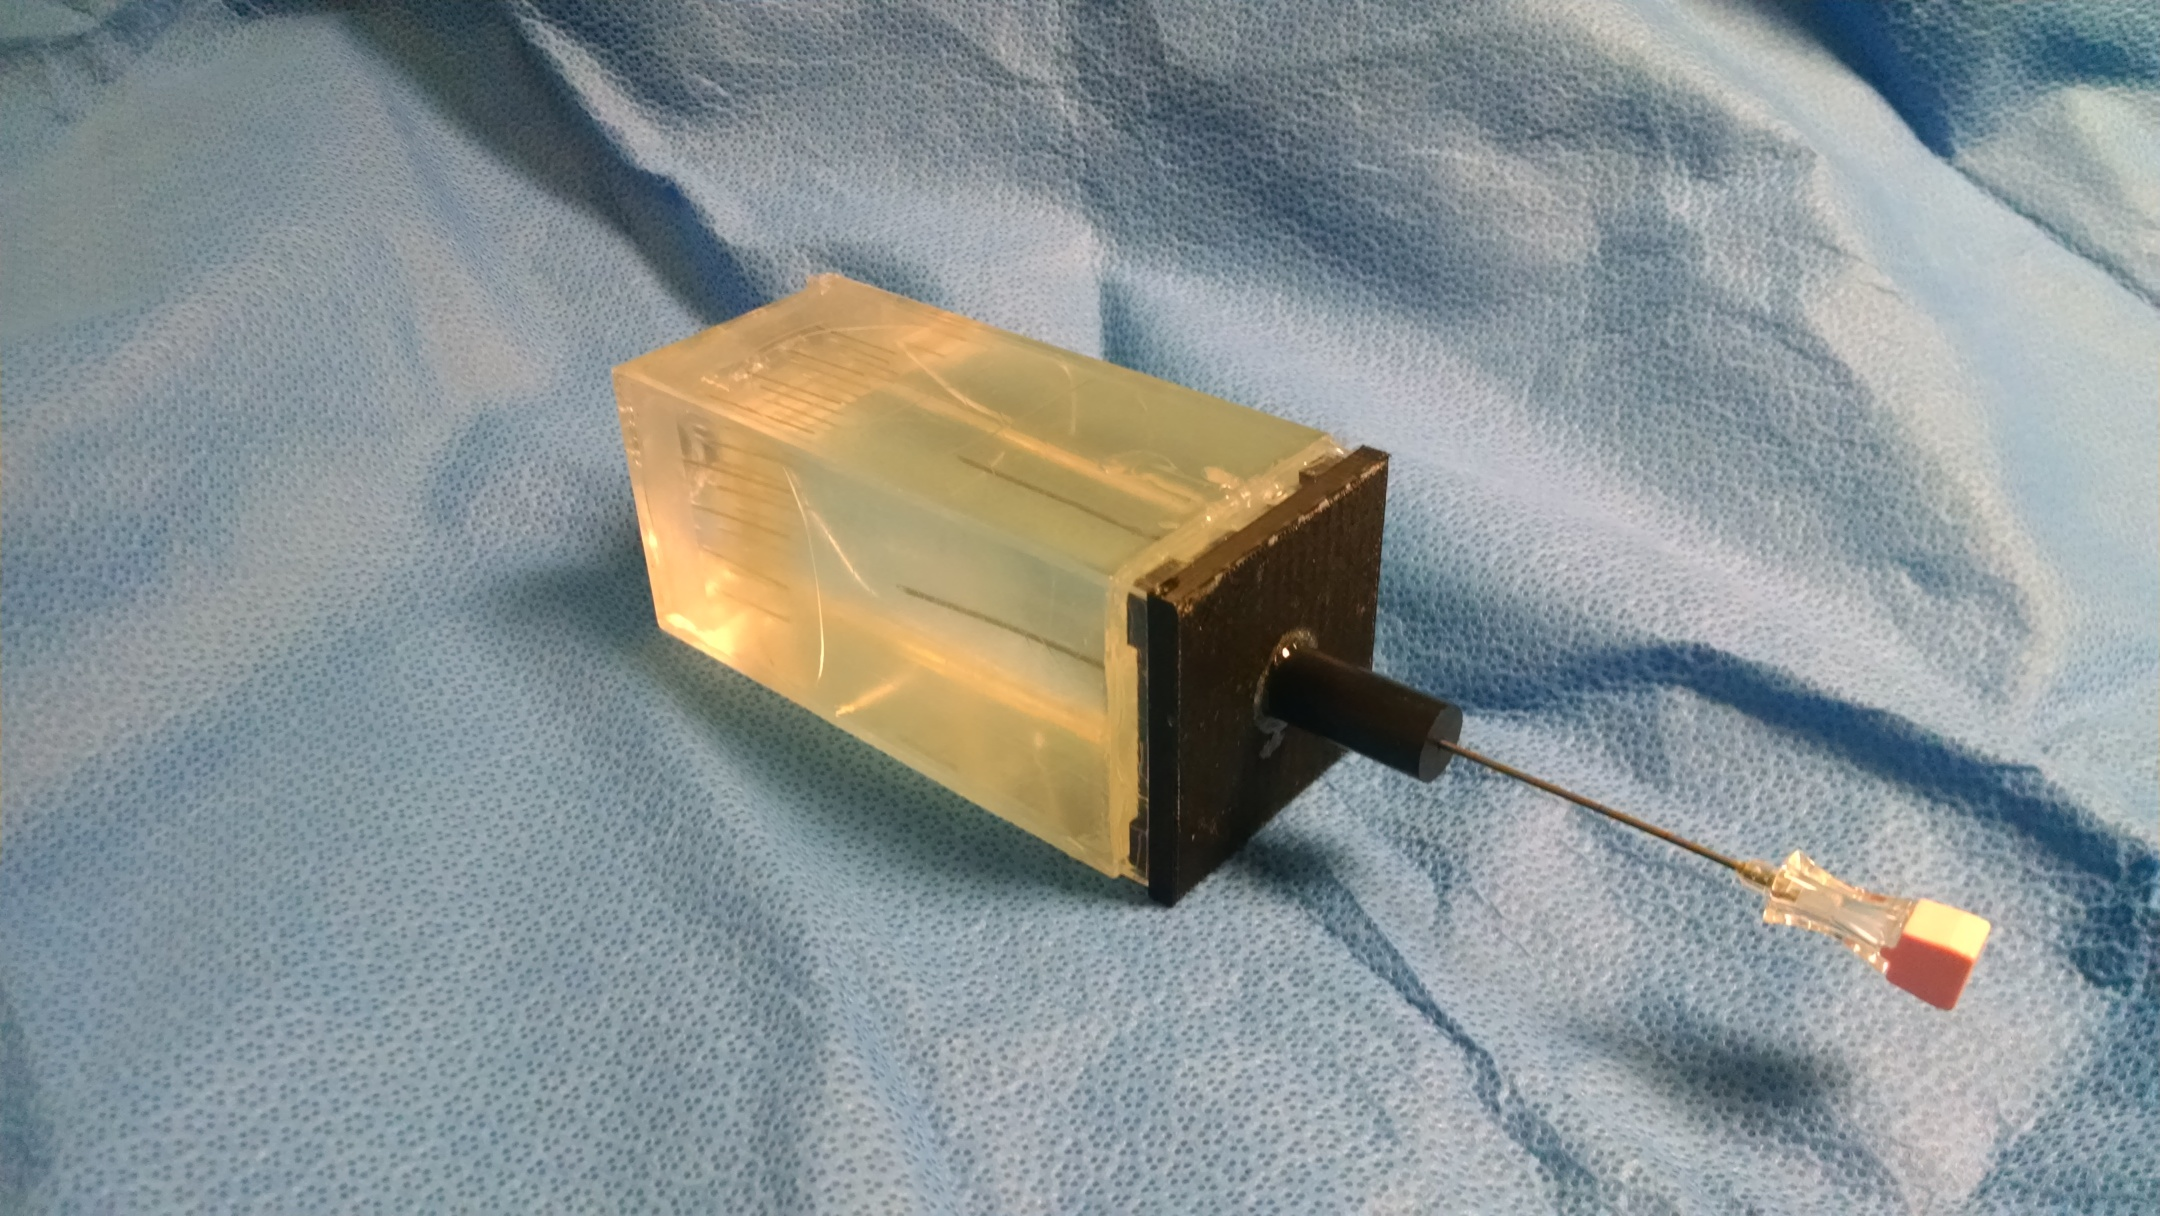
\includegraphics[width=1.0\textwidth]{Fig/chap5/phantom_with_needle_guide_small_2.jpg}
\caption{Tissue phantom with needle alignment frame and biopsy needle.}
\label{fig:needle_guide}
\end{figure}

\section{Results}

TODO: (Fu) "The model characterizes well the behavior of the needle with relatively small insertion distance (in Fig. 4.5, 4.6) and has a large error for large insertion depth, no matter the order of polynomial chosen, as noted in the discussion section. Is there any thought on how to improve the performance? If so, please include them in the discussion."

TODO: (Fu) "Is it possible to compare the result with a dynamic model of the needle and vision-based state estimation?"

The baseline for the position of the needle shaft in the phantom was established by segmenting the needle artifact via thresholding and computing the centroid of its cross section in each axial scan slice. Figure \ref{fig:seg_2001} shows the segmentation for the final step of the insertion, and Figure \ref{fig:ground_truth_2001} shows the positions of the centroids in successive axial planes. The error for each model is computed as the difference between the centroid coordinate and the modeled coordinate in each slice.

\begin{figure}[h]
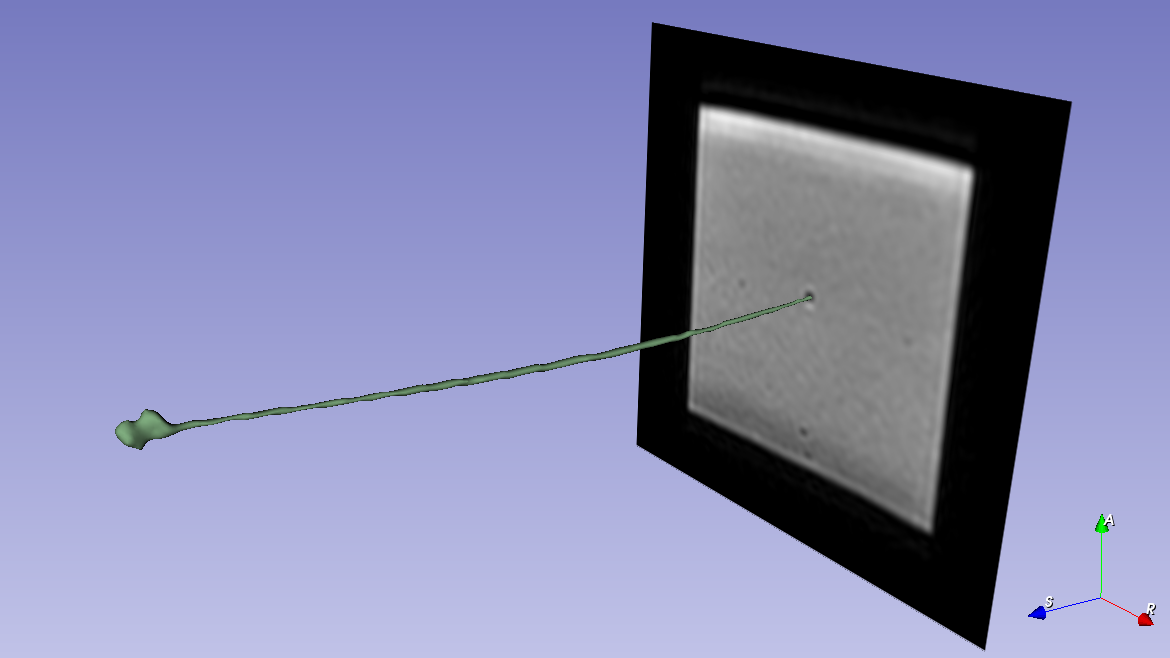
\includegraphics[width=1.0\textwidth]{Fig/chap5/segmented_artifact_2001.png}
\caption{Segmentation of needle artifact generated by thresholding MRI volume.}
\label{fig:seg_2001}
\end{figure}

\begin{figure}[h]
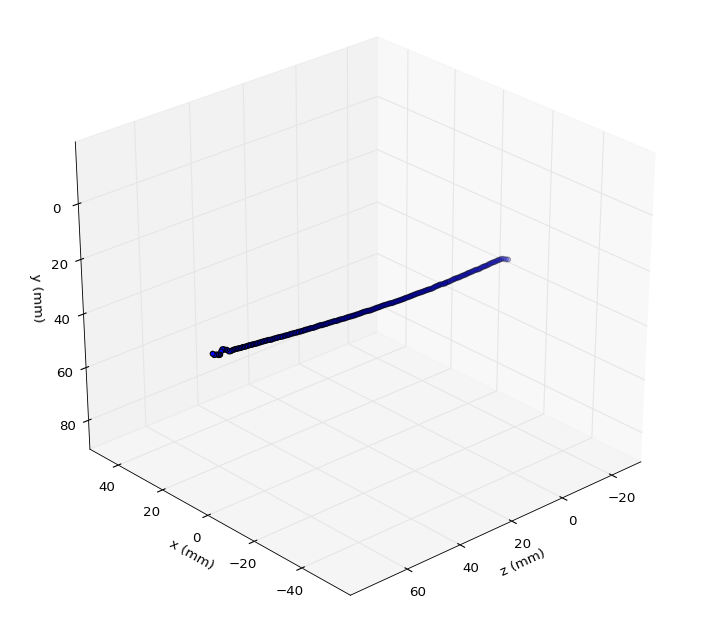
\includegraphics[width=1.0\textwidth]{Fig/chap5/neutral_axis_2001_b.png}
\caption{Baseline ground truth data, calculated from the centroids of the segmented artifact sectioned in the X-Y plane.}
\label{fig:ground_truth_2001}
\end{figure}

\subsection{Needle Localization at a Single Timestep}
\label{sec:mri_single_timestep}
At the start of curve optimization using data from an individual insertion step the needle is assumed to be a vector with magnitude matching the length of the needle. The sampling locations are offset from the estimated position of the needle tip by a user-configurable distance to avoid sampling points within the tip artifact. In this experiment the tip offset was 5mm, the sample spacing was 10mm, and the number of samples was 3. The models under comparison use 1st-, 3rd-, 5th-, and 7th-degree polynomials.

Figure \ref{fig:results_error_comparison} shows the relative error using a 1st-, 3rd-, 5th-, and 7th-degree polynomials. 

\begin{figure}[h]

\includegraphics[width=1.0\textwidth]{Fig/placeholder.png}
\caption{Magnitude of in-plane error over insertion for various degrees of polynomial.}
\label{fig:results_error_comparison}
\end{figure}

% \begin{figure}[h]
% \includegraphics[width=1.0\textwidth]{Fig/chap5/error_curvepoints_1501_1deg_3p_10mm.png}
% \caption{Magnitude of in-plane error over insertion depth using a linear model.}
% \label{fig:results_error_linear}
% \end{figure}

% \begin{figure}[h]
% \includegraphics[width=1.0\textwidth]{Fig/chap5/error_curvepoints_1501_3deg_3p_10mm.png}
% \caption{Magnitude of in-plane error over insertion depth for the needle mechanical model using a 3rd-degree polynomial.}
% \label{fig:results_error_3rd}
% \end{figure}

% \begin{figure}[h]
% \includegraphics[width=1.0\textwidth]{Fig/chap5/error_curvepoints_1501_5deg_3p_10mm.png}
% \caption{Magnitude of in-plane error over insertion depth for the needle mechanical model using a 5th-degree polynomial.}
% \label{fig:results_error_5th}
% \end{figure}

% \begin{figure}[h]
% \includegraphics[width=1.0\textwidth]{Fig/chap5/error_curvepoints_1501_7deg_3p_10mm.png}
% \caption{Magnitude of in-plane error over insertion depth for the needle mechanical model using a 7th-degree polynomial.}
% \label{fig:results_error_7th}
% \end{figure}

\subsection{Needle Localization at Sequential Timesteps}
Needle tracking in a sequence of images consists of repeated application of the method for an individual timestep described in \ref{sec:mri_single_timestep}. The optimized curve from the previous localization step is used as the initial estimate for the next localization step. The curve was a 5th-degree polynomial. Three sample points were selected, starting 5mm from the tip and spaced 10mm apart.

Figure \ref{fig:scan_slices} shows the positions of the scan planes and Figure \ref{fig:curve_points} shows points along the optimized curve for each insertion interval. Figure \ref{fig:curve_errors_fixed_spacing} shows the magnitude of error relative to the baseline for the optimized curve at each interval. Figure \ref{fig:curve_errors_variable_spacing} shows the magnitude of error when the spacing between the sample points is increased as the needle is inserted.

\begin{figure}[h]
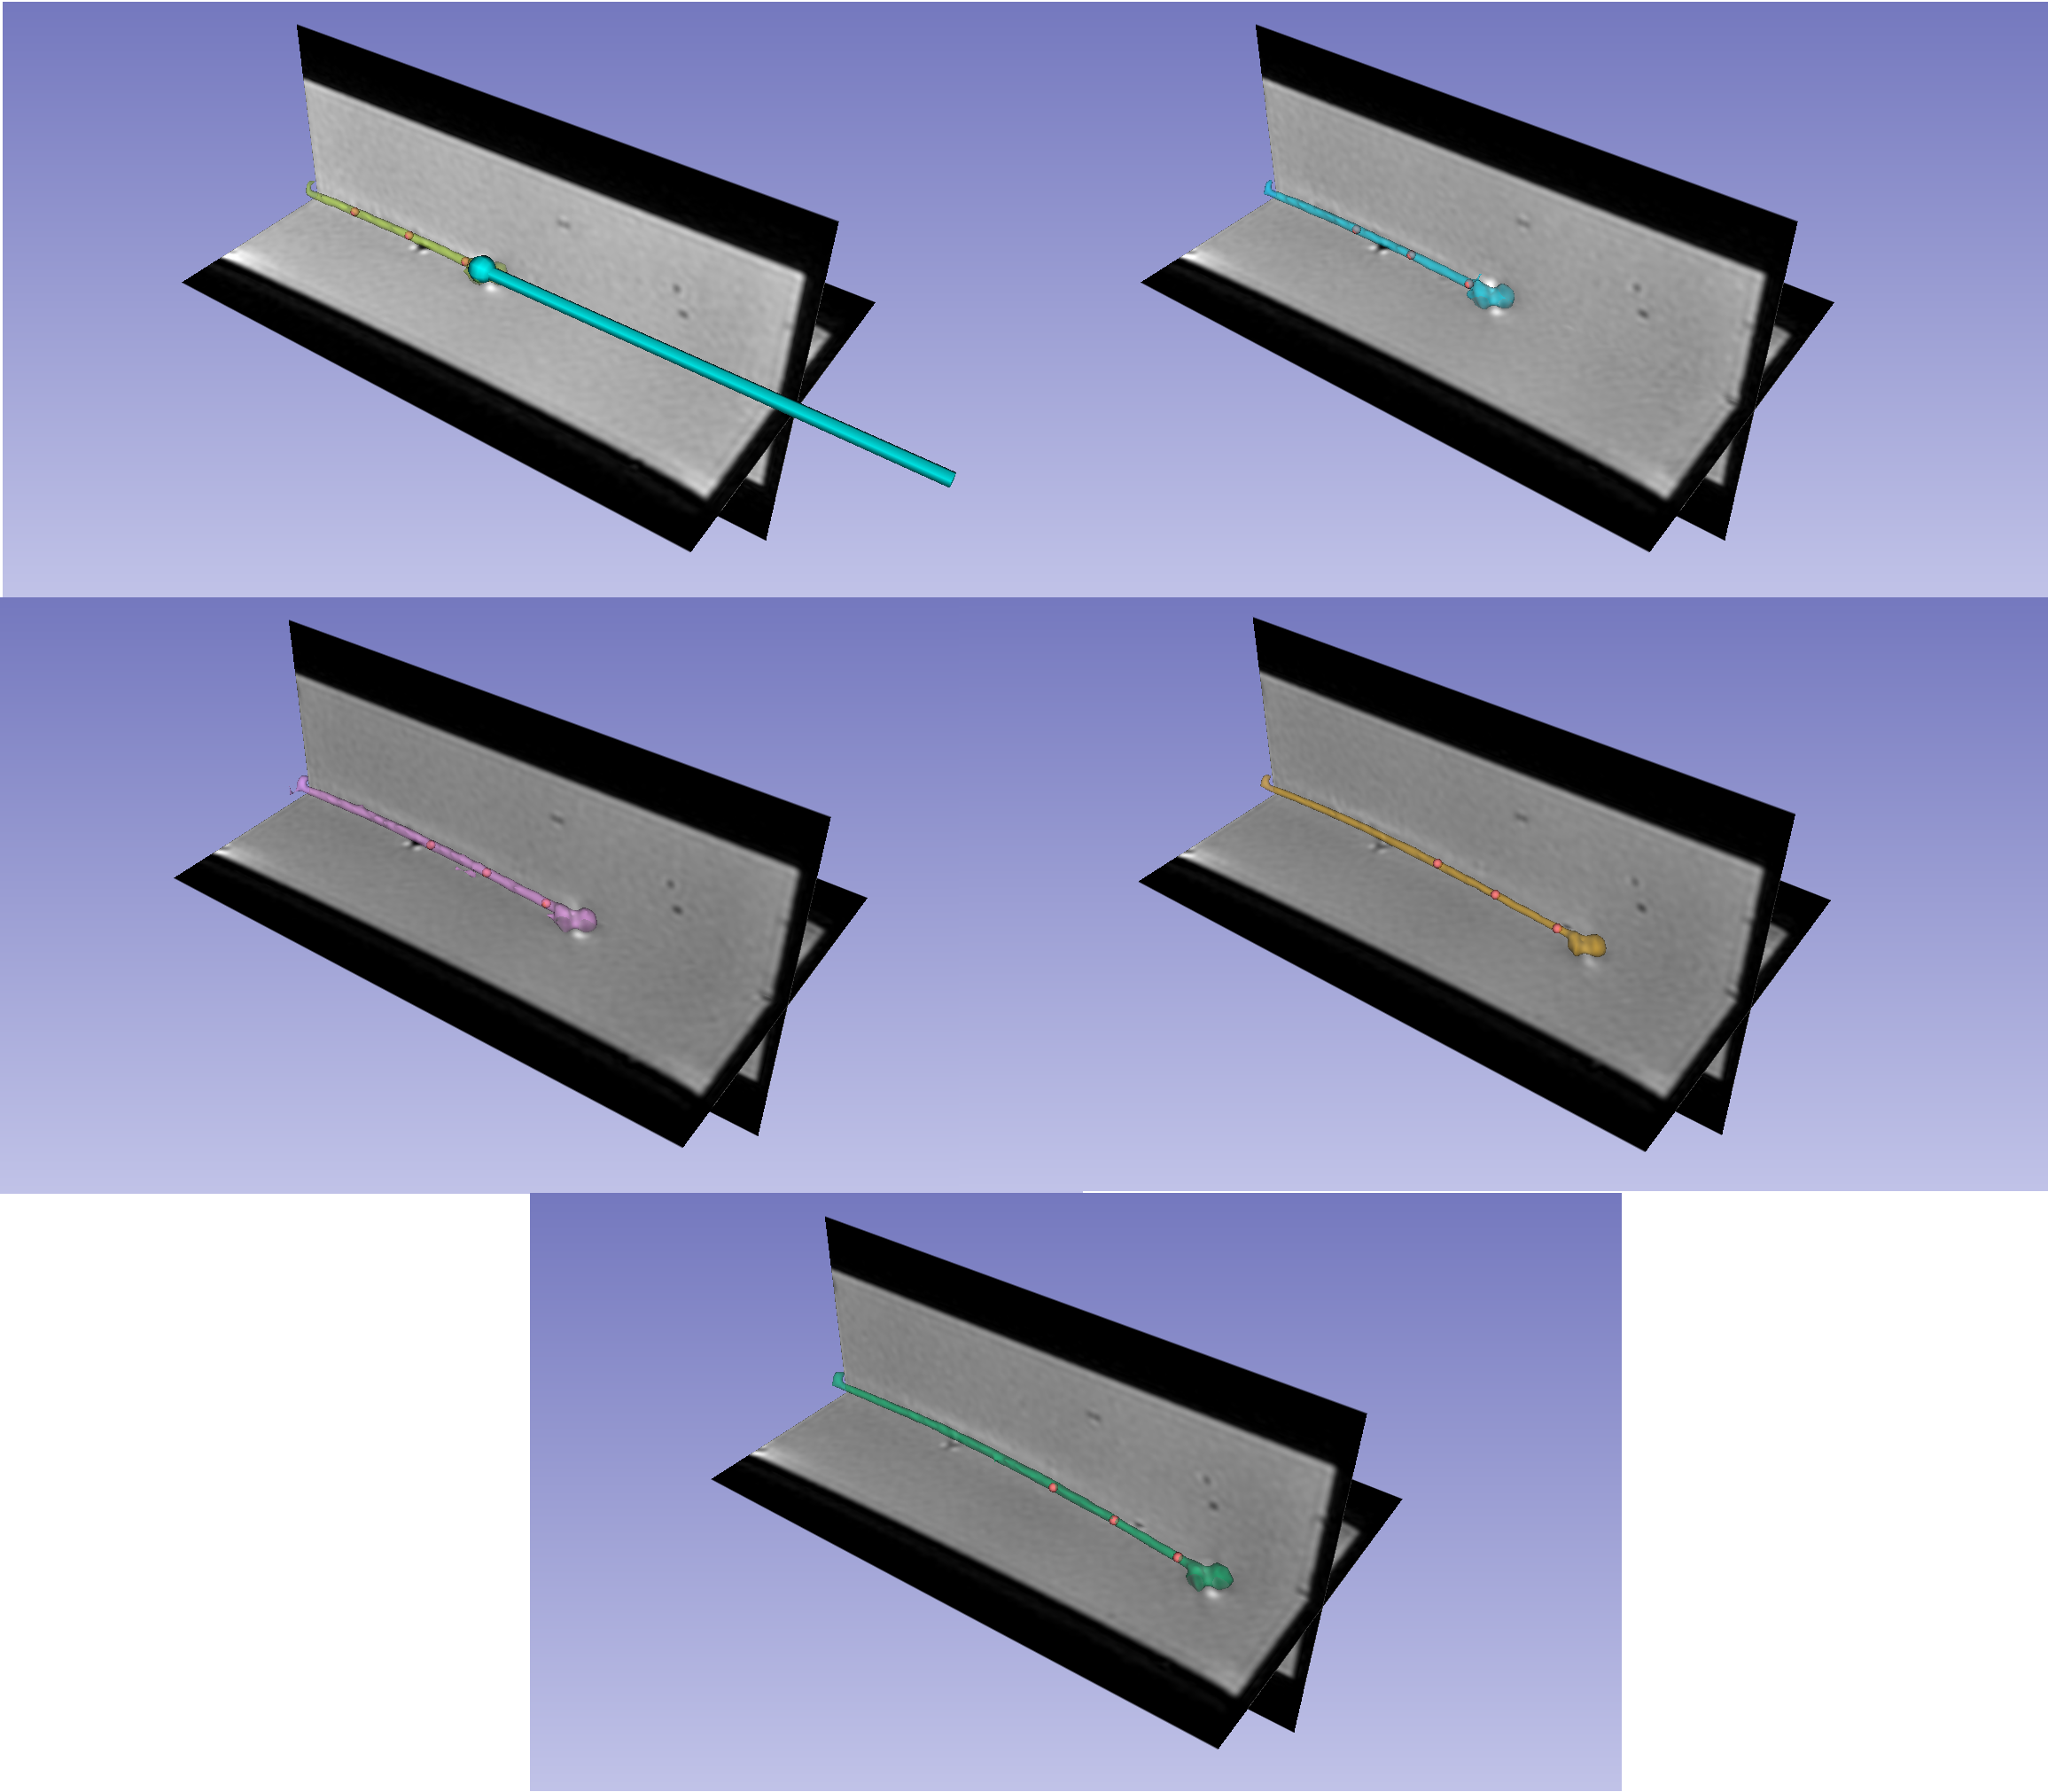
\includegraphics[width=1.0\textwidth]{Fig/chap5/scan_slices.png}
\caption{Positions of 2D scan planes at each insertion step, with segmented artifact.}
\label{fig:scan_slices}
\end{figure}

\begin{figure}[h]
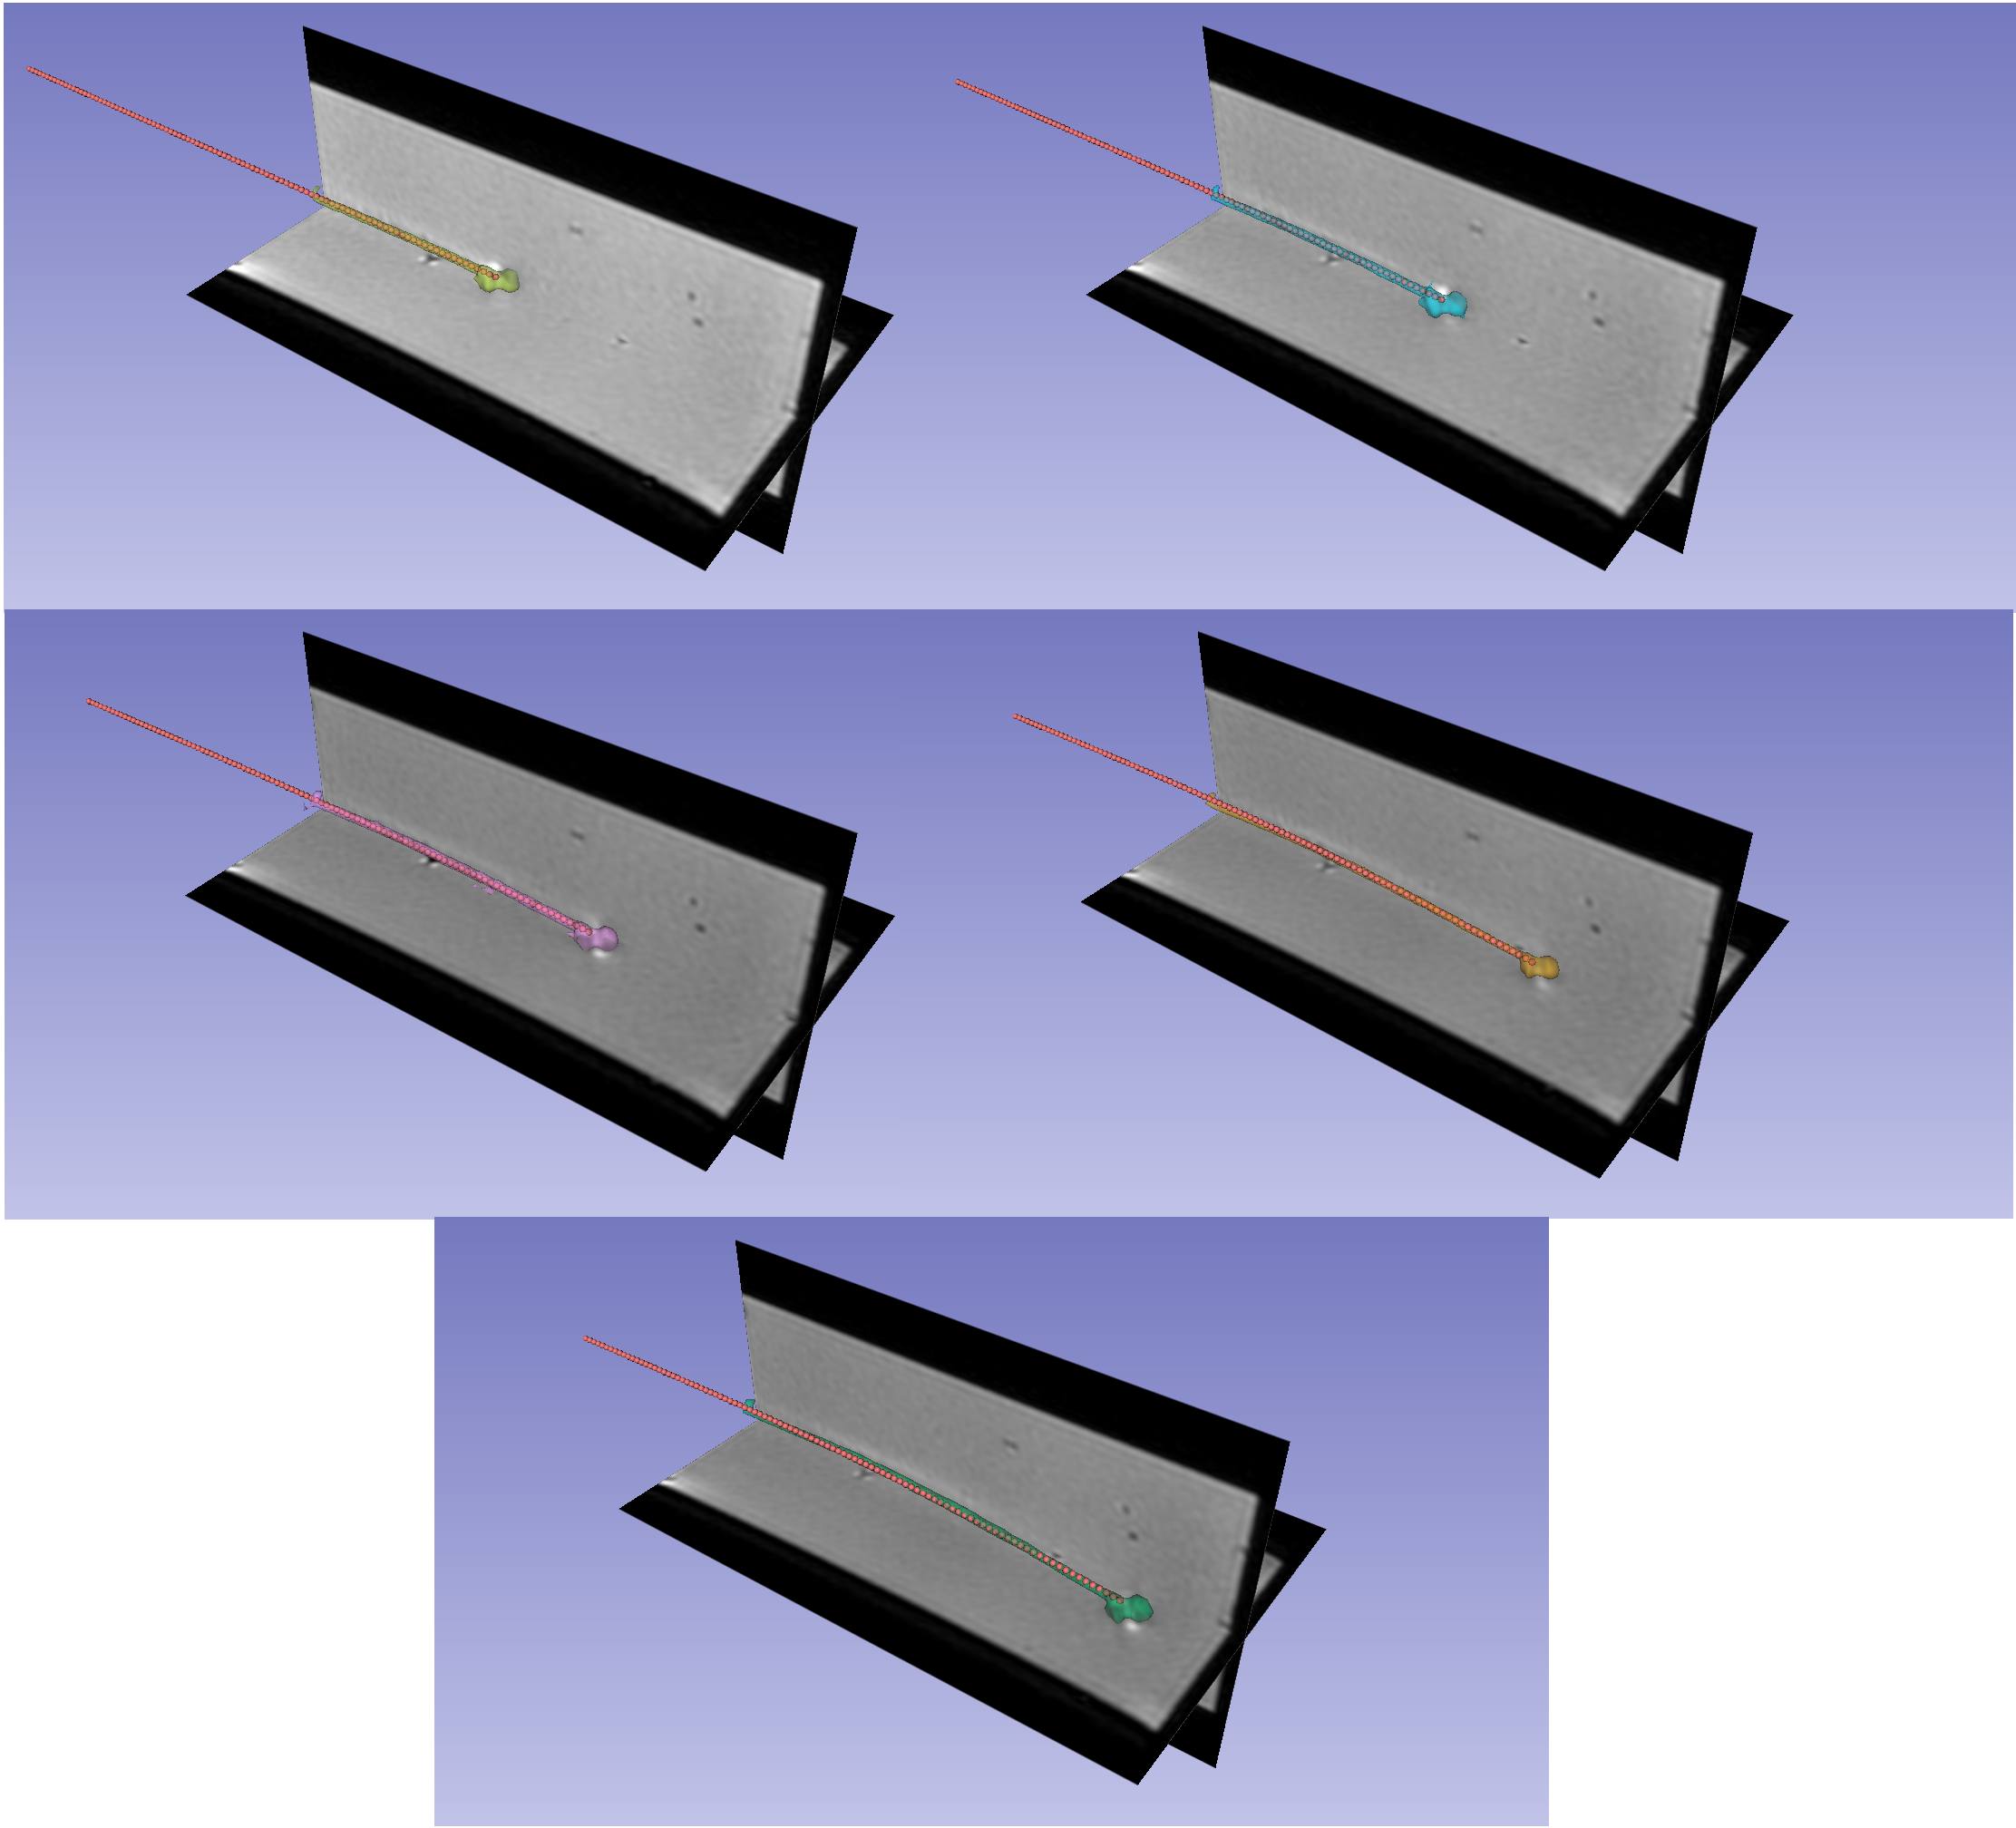
\includegraphics[width=1.0\textwidth]{Fig/chap5/insertions.png}
\caption{Modeled curve points at each insertion step, with segmented artifact.}
\label{fig:curve_points}
\end{figure}

\begin{figure}[h]
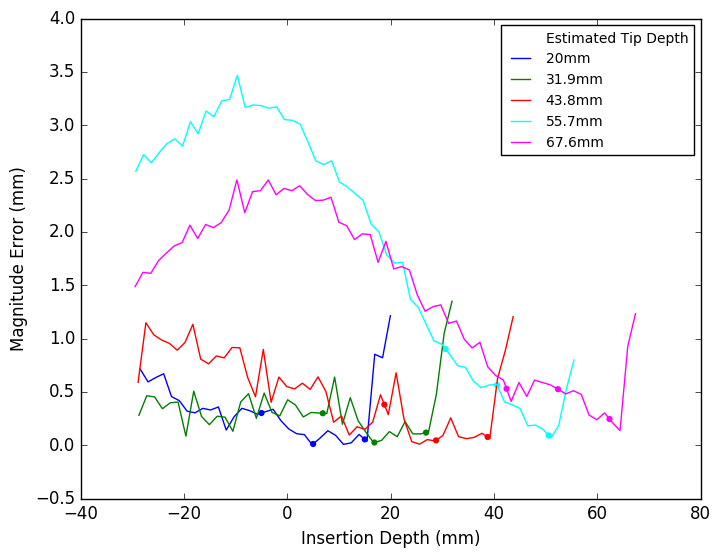
\includegraphics[width=1.0\textwidth]{Fig/chap5/error_curve_3_10.png}
\caption{Magnitude of error between the needle model and the artifact centroid. $\delta=5mm$, $k=3$, $d=10$}
\label{fig:curve_errors_fixed_spacing}
\end{figure}

\begin{figure}[h]
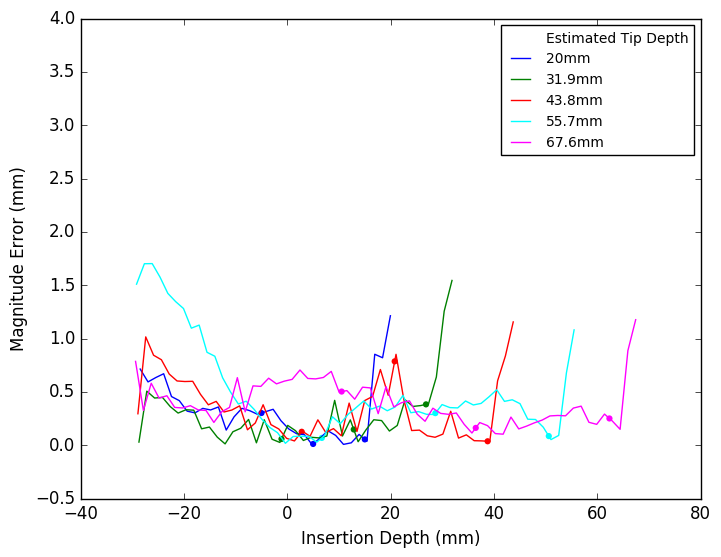
\includegraphics[width=1.0\textwidth]{Fig/chap5/error_curve_3_var.png}
\caption{Magnitude of error between the needle model and the artifact centroid. Each line is a different insertion step.}
\label{fig:curve_errors_variable_spacing}
\end{figure}



% Figures \ref{fig:results_error_poly_3rd} and \ref{fig:results_error_poly_7th} show the relative error using, respectively, a 3rd-degree and a 7th-degree polynomial least-squares fit. This model is a better fit than the linear fit, but the higher-degree polynomial overfits the small number of datapoints and introduces sharp turns that are not representative of the mechanical behavior of the needle. Additionally, the directions of these curves at the base and tip do not reflect the actual behavior of the needle.

% \begin{figure}[h]
% 
\includegraphics[width=8cm]{Fig/placeholder.jpg}
% \caption{Magnitude of in-plane error over insertion depth using a 3rd-order polynomial least-squares fit.}
% \label{fig:results_error_poly_3rd}
% \end{figure}

% \begin{figure}[h]
% 
\includegraphics[width=8cm]{Fig/placeholder.jpg}
% \caption{Magnitude of in-plane error over insertion depth using a 7th-order polynomial least-squares fit.}
% \label{fig:results_error_poly_7th}
% \end{figure}


% \begin{figure}[h]
% 
\includegraphics[width=8cm]{Fig/placeholder.jpg}
% \caption{Magnitude of needle tip pose orientation error for each type of needle model.}
% \label{fig:pose_error}
% \end{figure}
